\chapter{Background}\label{chapter:background}

The Zipfian distribution (also known as \textit {Zipf's Law}
 \cite{powersApplicationsExplanationsZipfs1998a}) is a power law; that is, 
 the relationship between the probability of an event and the quantity that 
 describes the event 
is given by an exponential factor \cite{newmanPowerLawsPareto2005}. A simple example of a power law is the relationship of the \textit{area of a square}, $A(x)$, and its 
\textit{side length}, $x$, given by $A(x) = x^2$. A formal definition is given below, parametrized by what we will
define as the \textit{skew} - $\alpha$.

\begin{equation}
    f(x) = C \cdot x^\alpha
    \label{eq:power-law}
\end{equation}

\paragraph{Zipf's Law} While a power-law, Zipf's is slightly different
 than the area of a square in that it is defined as a set of discrete values.
  For instance, when parsing a text and collecting the number of occurrences of 
  each word, there are only finitely many words. The same occurs for databases: a key to a table has only a finite number of values. Moreover,
 the law says that the word rank - a word's position or key in terms of popularity -
  is inversely proportional to its frequency, given a skew factor. Formally, 
  it is defined as follows:

\begin{equation}\label{eqt:zm_law}
    \textbf{frequency} \propto \frac{1}{\textbf{rank}^\alpha}
\end{equation}

An example is given in Figure \ref{fig:zipf_example}. A text was parsed and a 
list of top five most popular words has been compiled: "the", "a", "an", "of", "to".
The frequency is defined to be $freq(word) = \frac{occurences(word)}{\sum_{all words} occurences(words)}$.
 We observe that the frequencies sum up to $1$, and that the relationship
between rank and frequency is not linear, but closely resembles an exponential 
curve. 

\begin{figure}[t]
  \centering
  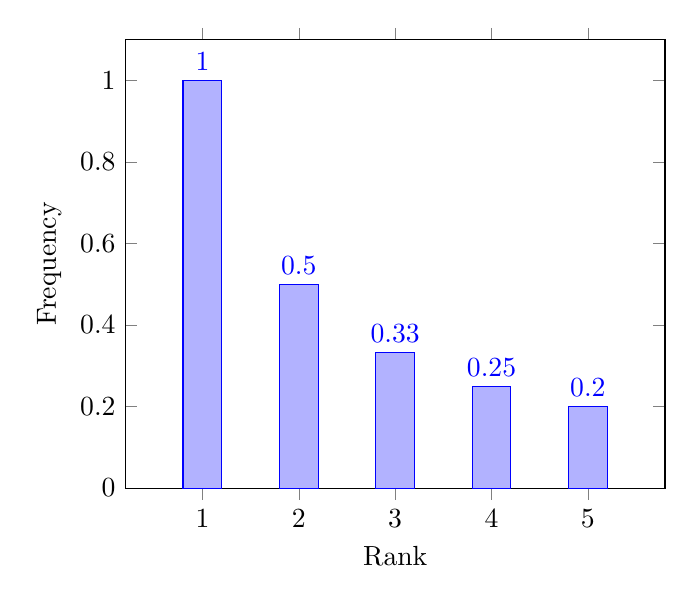
\begin{tikzpicture}
  \begin{axis}[
    ybar,
    bar width=14pt,
    enlarge x limits=0.2,
    symbolic x coords={1,2,3,4,5},
    xtick=data,
    xlabel={Rank},
    ylabel={Frequency},
    ymin=0, ymax=1.1,
    nodes near coords,
    ]
    \addplot coordinates {
      (1,1)     
      (2,0.5)   
      (3,0.333) 
      (4,0.25)   
      (5,0.2)    
    };
  \end{axis}
\end{tikzpicture}

  \caption{Example of a Zipfian distribution}
  \label{fig:zipf_example} 
\end{figure}

\paragraph{The generalized Zipfian} The previous example and intuition are helpful in 
understanding the pattern that this law presents, however, it is necessary to define 
it more deeply. From now on, the following conventions will be used:

\begin{itemize}
    \item $N$ - The support size of the distribution (e.g. \textit{number of different words})
    \item $k$ - The rank of the \textit{variate}\footnote{this is used interchangebly with \textit{sample}} (e.g. \textit{rank of word})
\end{itemize}

Since the aim is generating variates according to this law, it is necessary to
 treat the \textit{generalized Zipfian} as a statistical distribution. Below follows its
\ac{PMF}:
\begin{equation}\label{eqt:zm_prob}
    f(k, N, \alpha) := 
 \begin{cases} 
      \frac{1}{H_{N,\alpha}} \frac{1}{k^\alpha} & 1 \leq k \leq N \\
      0 & k < 1 \, \text{or} \, N < k 
   \end{cases}
\end{equation}

The term $H_{N,\alpha}$ is defined as the \textit{generalized harmonic number} \cite{newmanPowerLawsPareto2005}, acting as the normalizing constant $C$ 
seen in \ref{eq:power-law} and ensuring the \ac{PMF} sums to $1$. It is defined as:

\begin{equation}\label{eqt:generalized_hn}
    H_{N, \alpha} = \sum_{k = 1}^{N} \frac{1}{k^\alpha}
\end{equation}

As done before with Zipf's Law, the \textit{Zipfian} distribution is plotted in Figure \ref{fig:zipf_pmf} as a line plot, this time with a \textit{support size} of $100$ distinct words. 
Now that all relevant terms are defined, we turn to the original problem of generating \textit{samples}.

\begin{figure}[t]
    \centering
    \begin{tikzpicture}
    \begin{axis}[
        xlabel={$k$},
        ylabel={$P(X=k)$},
        grid=both,
        thick,
        ymin=0,
        ymax=0.2,
        xtick distance=10,
    ]
    
    \pgfplotstableread[col sep=comma]{data/zipf_pmf.csv}\datatable  
    \addplot table[x=k, y=PMF] {\datatable};
    \end{axis}
\end{tikzpicture}
    \caption{Probability Mass Function of a Zipfian distribution with $N = 100$ and $\alpha = 1$}
    \label{fig:zipf_pmf}
\end{figure}

\section{Discrete Variate Generation}
The goal of \textit{discrete variate generation} is to produce a set
 $\tilde{X}$ of $m$ variates contained in the \textit{support interval} $[0,N]$, 
 such that $freq(x_i) \sim Dist(\alpha)$ for $i \in [0,m]$. In other words,
  the samples follow a given distribution $Dist(\alpha)$. To achieve this, all sampling algorithms use 
an random \textit{uniform} distribution $U$, and transform  these uniform \textit{samples} into the 
target samples \cite{kuhlHistoryRandomVariate2017}. As distributions 
have different properties, some sampling methods are better than others for a particular distribution. Knowing this, the discussion is restricted to the algorithms listed below, as literature
confirms these methods are better than alternatives (see \cite{devroyeDiscreteUnivariateDistributions1986,kronmalAliasMethodGenerating1979,kuhlHistoryRandomVariate2017}).

\begin{enumerate}
    \item Rejection Sampling \cite{devroyeDiscreteUnivariateDistributions1986}
    \item Rejection-Inversion Sampling \cite{hormannRejectioninversionGenerateVariates1996}
    \item Condensed Table Lookup \cite{marsagliaFastGenerationDiscrete2004}
    \item Approximative sampling \cite{grayQuicklyGeneratingBillionrecord1994}
\end{enumerate}

The first two methods, \textit{Rejection Sampling} and \textit{Rejection-Inversion Sampling}, are \textbf{exact}, whereas the last two, \textit{Condensed Table Lookup}
and \textit{Approximative Sampling}, are \textbf{approximations}. Consequently, given enough samples, the first two should converge to a \textit{Zipfian} distribution if implemented correctly,
whereas the latter two might have systematic deviations \cite{leydoldErrorDetectionNonUniforma}. The following subsections will explain each algorithm.

\subsection{Rejection Sampling}\label{subsec:rejection_sampling}
Rejection sampling works by \textit{rejecting} samples from a \textit{uniform}
 distribution using a \textit{bounding function} to decide which samples are kept 
and which are thrown away. A good example is a dartboard, onto which darts are 
thrown at random. If the target distribution is normal, we draw its contour
(the \textit{bounding function}) in the dartboard and \textit{accept}
 the darts that fall below it and \textit{reject} the ones above. 
The graphs in Figure \ref{fig:rejection_sampling} illustrate this principle well 
- blue points are accepted darts, whereas red points are the rejected ones.

\begin{figure}[ht]
    \centering
    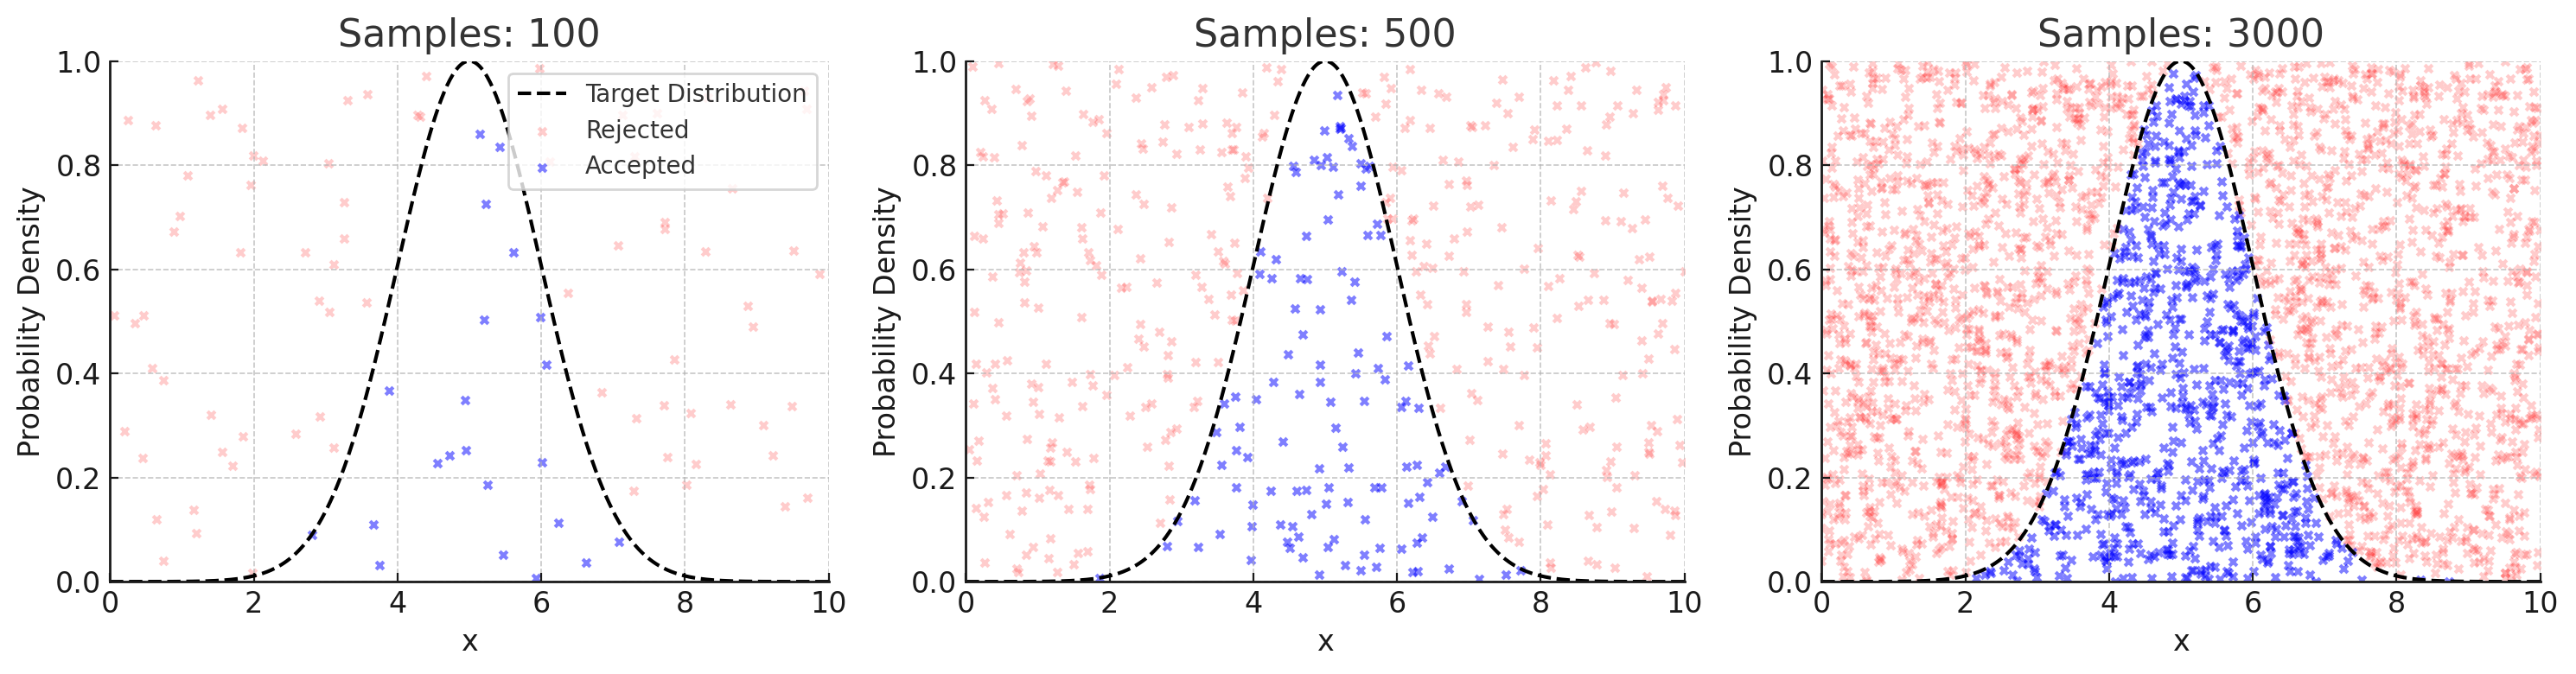
\includegraphics[width=\linewidth]{figures/rejection_sampling.png}
    \caption{To generate these graphs, a random uniform sample is taken for the x-axis as well as another normalized one for the y-axis.}\label{fig:rejection_sampling}
\end{figure}

Similar to the normal distribution, a \textit{bounding function} is chosen for the \textit{Zipfian}: $1/k^{-\alpha}$. This function is easier to determine than
the \ac{PMF} in Equation \ref{eqt:zm_prob}, as we skip the computationally expensive normalization constant. The only requirement on this function is that it should 
\textit{be greater up to a constant factor} than the original \ac{PMF}. A disadvantage of 
this method is that two random samples are required: one for the x-axis, another for the y-axis.

\subsection{Rejection-Inversion Sampling}\label{subsec:rejection_inversion}
Due to Hörmann and Derflinger \cite{hormannRejectioninversionGenerateVariates1996}, this method
 is a more efficient version of the Rejection Sampling method. 
It is based on the following observations regarding the naive rejection method:
\begin{itemize}
    \item A naive rejection algorithm requires two samples to generate the target variate.
    \item The Zipfian is bounded by a monotonically decreasing and convex function, which makes it possible to invert the bounding function.
\end{itemize}

These two observations lead to the following principle:

\vspace{0.3cm}

\fbox{
    \parbox{0.83\linewidth}{
        Generate a random variate $u$ from the uniform distribution $U(0,1)$ and invert the bounding function to find the corresponding $x = H^{-1}(u)$.
        Define a bounding area around the nearest integer $k$ (with radius $a$).
        Accept $X$ as a sample if $x \geq x_k$ and $x \leq k + a $. Otherwise, reject it.\footnotemark
    }
}
\footnotetext{This is a simplified version of the algorithm. For a more detailed explanation, see \cite{hormannRejectioninversionGenerateVariates1996}}
\vspace{0.3cm}

To visualize the principle used, consider Figure \ref{fig:rejection_inversion}: After $k$ was found using the inversion method, the bounding area is defined for radius $a$. 
Therefore an interval beginning at $k - a$ and ending at $k + a$ is defined, then used to accept or reject $x$. Typically, $a$ is chosen to be $1/2$ \cite{hormannRejectioninversionGenerateVariates1996}.

\begin{figure}[t]
    \centering
    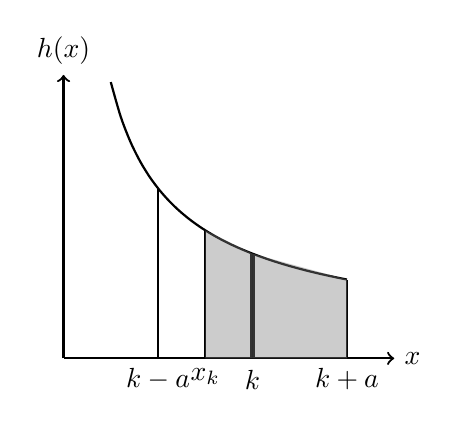
\begin{tikzpicture}[scale=1.2]
    % Axes
    \draw[thick,->] (0,0) -- (3.5,0) node[right] {$x$};
    \draw[thick,->] (0,0) -- (0,3) node[above] {$h(x)$};

    \draw[thick, domain=0.5:3, smooth, variable=\x] plot ({\x}, {1.8/\x^(0.7)});

    % Vertical lines
    \draw[thick] (1,0) node[below] {$k-a$} -- (1,{1.8});
    \draw[thick] (1.5,0) node[below] {$x_k$} -- (1.5,{1.8/(1.5^0.7)});
    \draw[ultra thick] (2,0) node[below] {$k$} -- (2,{1.8/(2^0.7)});
    \draw[thick] (3,0) node[below] {$k+a$} -- (3,{1.8/(3^0.7)});

    % Shaded areas (rejection and acceptance)
    \fill[gray,opacity=0.4] (1.5,0) -- (1.5,{1.8/(1.5^0.7)}) -- (2,{1.8/(2^0.7)}) -- (2,0) -- cycle;
    \fill[gray,opacity=0.4] (2,0) -- (2,{1.8/(2^0.7)}) -- (3,{1.8/(3^0.7)}) -- (3,0) -- cycle;

\end{tikzpicture}

    \caption{Rejection-Inversion Sampling for a Zipfian distribution}\label{fig:rejection_inversion}
\end{figure}

\subsection{Condensed Table Lookup}\label{subsec:condensed_table}
An alternative to exact methods is computing probabilities of a function according to a \ac{PMF} for all \textit{ranks} in the domain and storing them in a table. Since this 
probability is defined in an interval $[0,1]$, it is possible to take a random \textit{uniform} sample from the interval $[0,1]$ and look up the entry stored at the matching probability.
This sampling technique is called a \textit{table lookup} method \cite{marsagliaFastGenerationDiscrete2004}. Consider Figure \ref{fig:lookup_table}: 
A sample from an \textit{uniform} distribution (the implementation is a \ac{PRNG}) is taken and used to find the corresponding index in the table.

\begin{figure}[h]
    \centering
    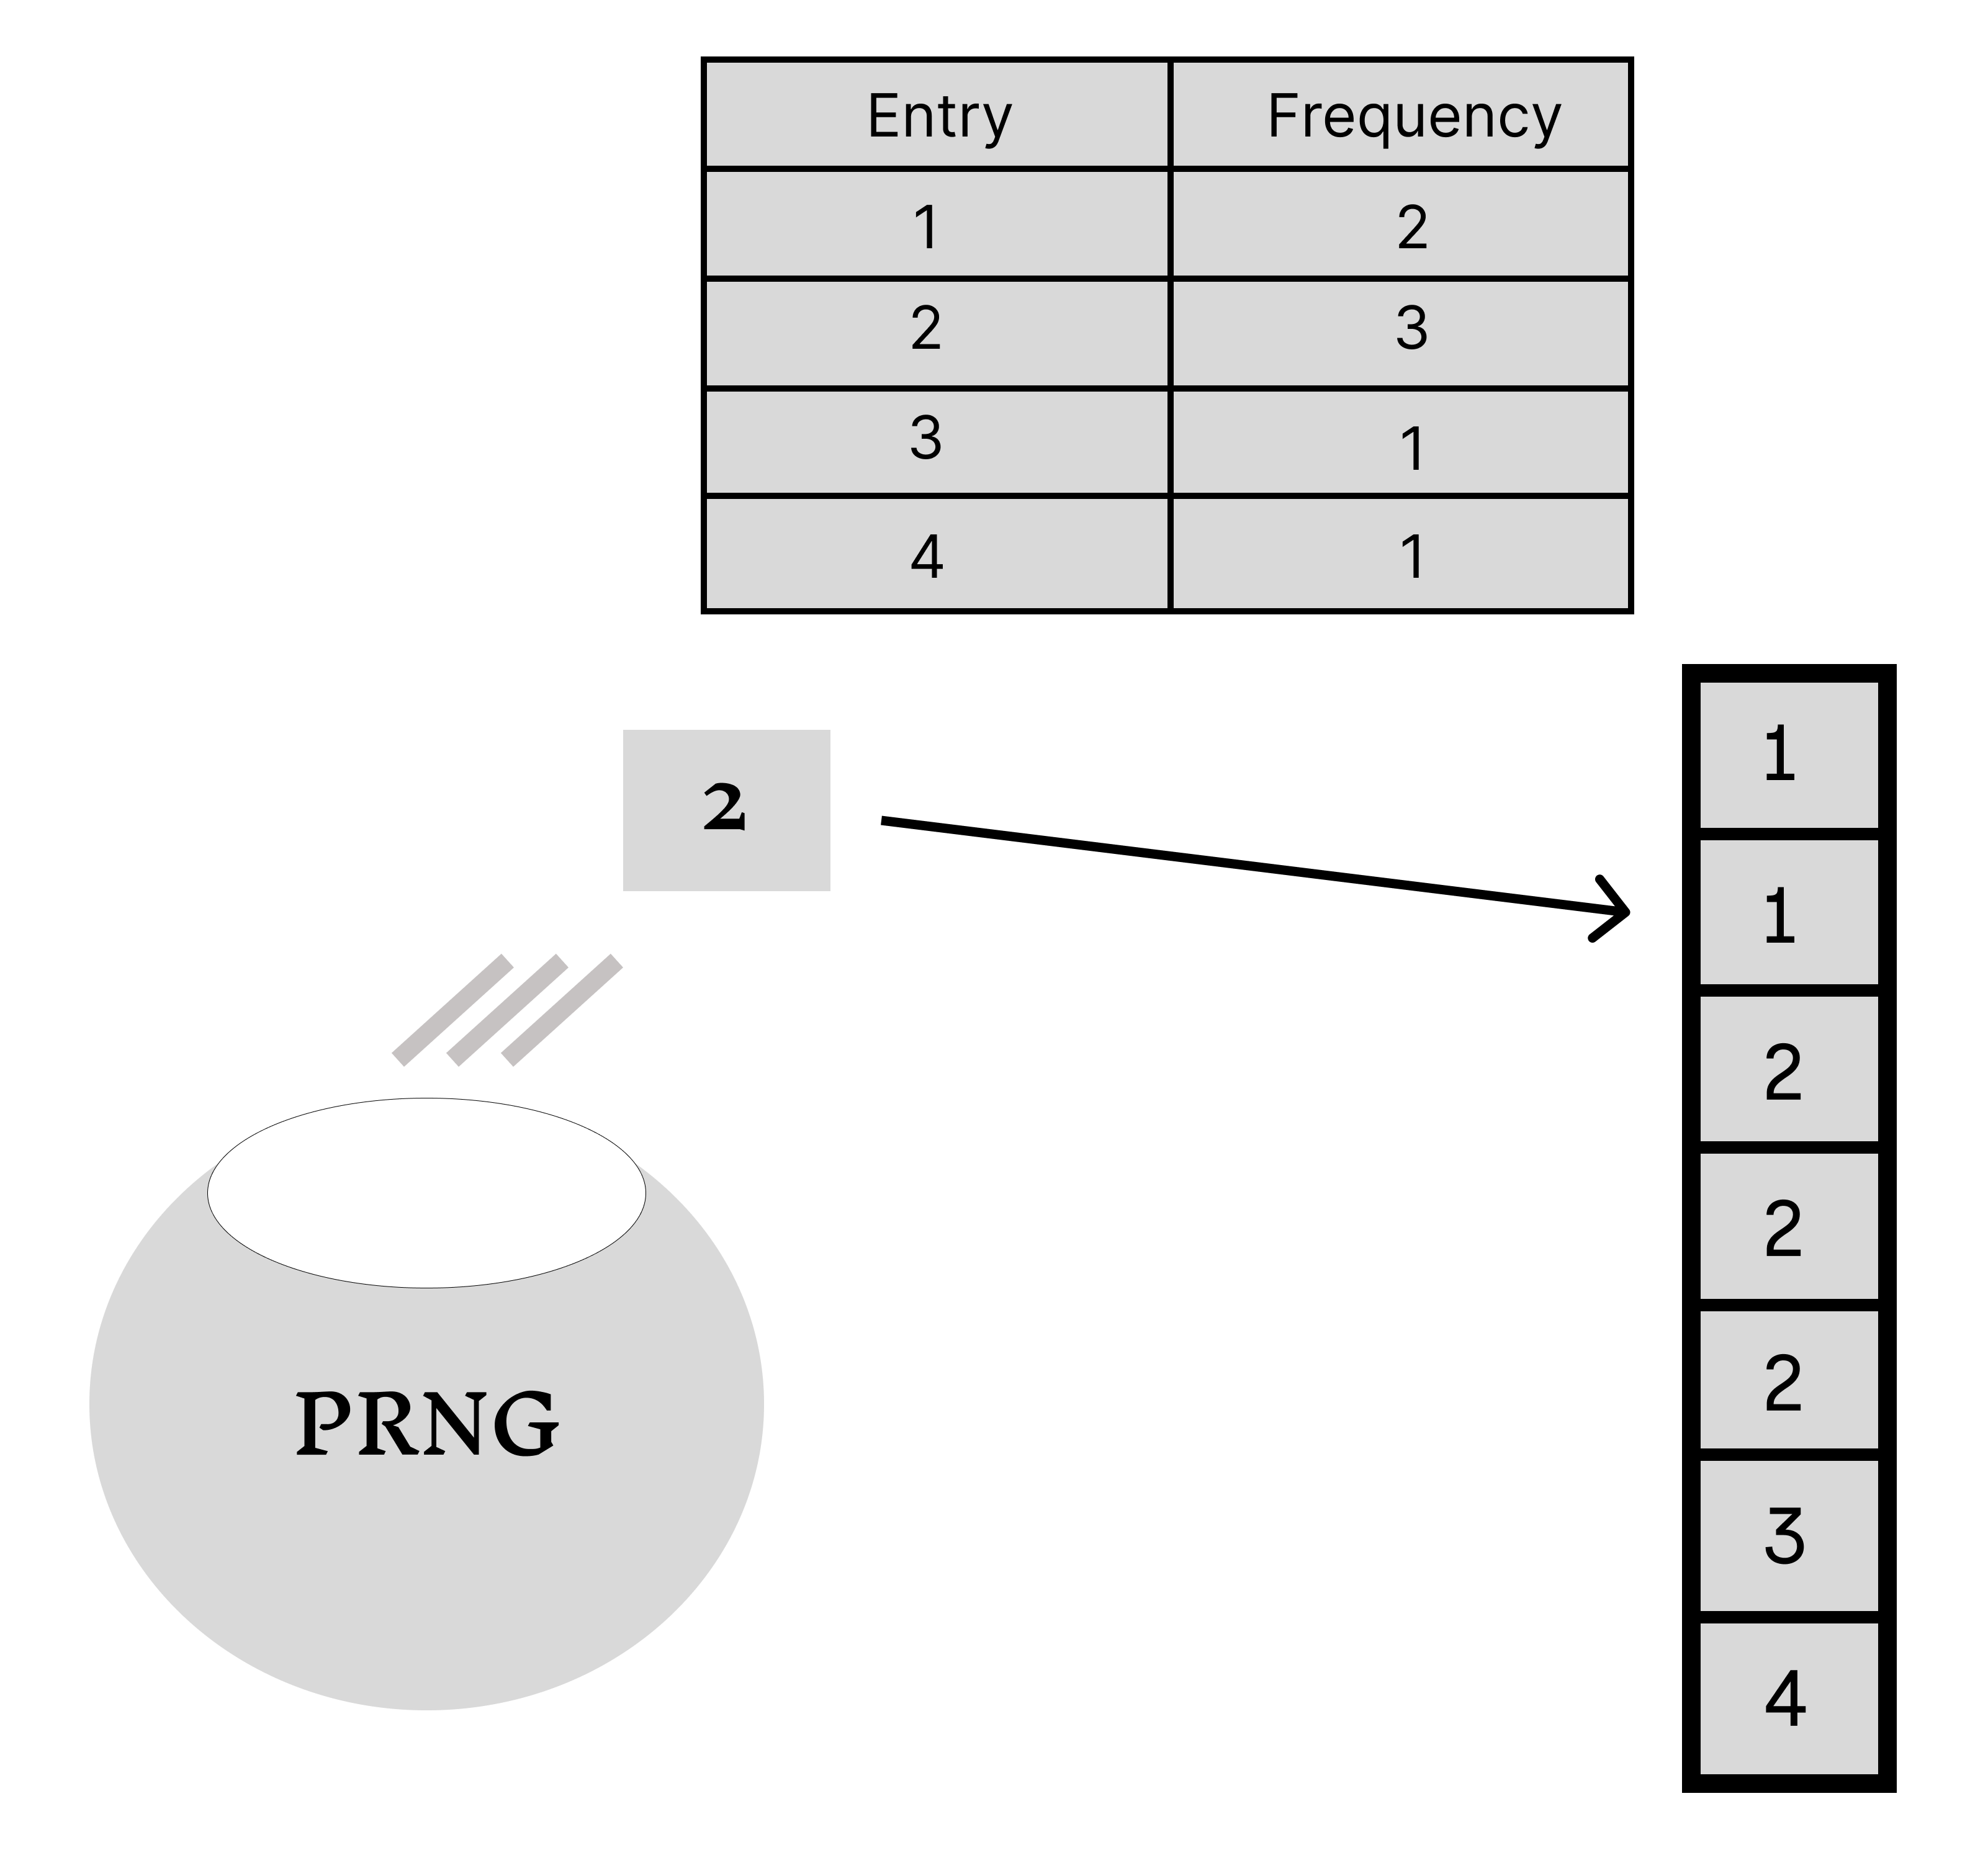
\includegraphics[width=9cm]{figures/marsaglia.png}
    \caption{The table contains the frequency of each index, whereas the array is populated 
    with as many entries as there are occurrences of each index. The sample "2" was generated, which is used to access the second position in the array}
    \label{fig:lookup_table}
\end{figure}

One limitation of this approach is the size of the array being in $O(n)$, which is not feasible for large \textit{support} $N$. 
To circumvent this, Marsaglia and Tsang proposed a \textit{condensed table lookup method} \cite{marsagliaFastGenerationDiscrete2004}, which 
works based on the principle exposed in the table below.

\vspace{0.2cm}
\fbox{
    \parbox{0.83\linewidth}{
        A floating-point number $p$ with $d$ decimal places can be used to represent a probability. For example, assuming $d = 2$, 
        the entry one from the last figure has probability $p(1) = 0.28$. To realize this probability, a table of size $10^2$ is required. 
        In order to achieve reasonable precision, a table of size in the magnitude of $10^{10}$ would be required, which would be unfeasable.
        Alternatively, less space can be used by breaking this table down to $d$ smaller tables. 
        To do this, each probability gets split into $d$ digits $m$, which respectively get $m$ entries in the corresponding table.  Now, generating a uniform integer from the interval $[1,100]$, it is possible to access the correct table and generate the variate.
        \footnotemark
    }
}
\vspace{0.2cm}
\footnotetext{This is a simplified version of the algorithm. For a more detailed explanation, see \cite{marsagliaFastGenerationDiscrete2004}}

\subsection{Approximation Sampling}\label{subsec:jim_gray}
Due to Gray \cite{grayQuicklyGeneratingBillionrecord1994}, this method is a fast approximation of the \textit{Zipfian's} tail and the generalized harmonic number.
The first few probabilities are calculated precisely and normalized by the approximated $H_{N,\alpha}$, while an exponential curve approximates the tail. 
A uniform sample is then used to generate a \textit{Zipfian} variate using inversion.
Figure \ref{fig:jim_gray} makes this idea clear by having two different areas along the x-axis. 

\begin{figure}[h]
    \centering
    \begin{tikzpicture}
    \begin{axis}[
        axis lines=left,
        xmin=0, xmax=30,
        ymin=0, ymax=0.05,
        ytick={0, 0.005, 0.01, 0.03, 0.05},
        yticklabels={0.5\%,1\%, 3\%, 5\%},
        xtick={1, 2, 3, 5, 10, 20, 30, 50},
        height=6cm,
        width=10cm,
        ybar,
        bar width=8pt,
        ymajorgrids=false,
        grid style=dashed,
        ylabel near ticks,
        xlabel near ticks,
        tick label style={font=\small}
    ]

    % Bar plot
    \addplot[ybar, fill=white] coordinates {
        (1, 0.05)
        (2, 0.035)
        (3, 0.025)
        (4, 0.017)
        (5, 0.015)
    };

    % Line plot
    \addplot[smooth, thick] coordinates {
        (5.5, 0.015)
        (10, 0.007)
        (20, 0.003)
        (30, 0.001)
    };

    \end{axis}
\end{tikzpicture}
    \caption{Jim Gray's method for generating samples from a Zipfian distribution}\label{fig:jim_gray}
\end{figure}

The mathematical description of this method is not quite straightforward and is omitted here. For a more detailed explanation, see \cite{grayQuicklyGeneratingBillionrecord1994,knuthArtComputerProgramming1997}.

\paragraph{Summary} As all generation techniques were described, the question remains how to evaluate them for accuracy compared with 
the theoretical probability values yielded by the \ac{PMF} in Equation \ref{eqt:zm_prob} - even for \textit{exact} methods. As these methods are developed, some assumptions
\cite{leydoldErrorDetectionNonUniforma} are taken that might not hold up in the computers used to generate these variates:

\begin{itemize}
    \item There exists a perfectly uniform generator that produces a sequence of \textit{independent} random variables uniformly distributed in $(0,1)$
    \item Computers can save and manipulate real numbers
\end{itemize}

Both of these assumptions cannot be fulfilled. First, the \textit{number generators} used are only pseudo-random \cite{kuhlHistoryRandomVariate2017} and might
have biases and produce correlated subsequences. For the second, computers only have limited precision, and computing terms such as the \textit{generalized harmonic number} suffer from
imprecisions caused by \textit{roundups} and \textit{cutoffs} \cite{leydoldErrorDetectionNonUniforma}. Some distributions such as \textit{power laws} worsen this issue \cite{radicchiUnderestimatingExtremeEvents2014}. Therefore,
we introduce a diverse set of criteria in the following sections for identifying correct implementations and measuring their errors:

\begin{itemize}
    \item Maximal absolute \ac{CDF} difference
    \item Sum of absolute \ac{PMF} differences
\end{itemize}

\section{Error Metrics}
To compare the different methods introduced previously, it is imperative to first define the framework used to evaluate them. Some principles can be applied from the literature
\cite{clausetPowerlawDistributionsEmpirical2009,leydoldErrorDetectionNonUniforma,monahanAccuracyRandomNumber1985}:

\begin{mdframed}
        \begin{enumerate}
            \item Calculate the theoretical distribution for the given parameters: $N$ - support size and $\alpha$ - skew.
            \item Generate an empirical distribution using the algorithms described earlier.
            \item Use a \textbf{goodness-of-fit test} to compare the generated distribution to the theoretical one.
        \end{enumerate}
        \label{box:accuracy}
\end{mdframed}

This framework assumes a "black-box" view of the generating processes and treats the generated samples as a dataset that should be fitted to the theoretical Zipfian. 
At the center of this comparison is a \textbf{goodness-of-fit test}, which tells whether the empirical distribution matches the expected distribution closely enough.
As such, the test requires a \textit{comparison metric} between the two distributions - a function that takes two distributions and returns a number that quantifies their dissimilarity. 
Let us look at the example given in Figure \ref{fig:accuracy-measure}. If the blue curve represents the theoretical distribution and the orange curve is the empirical one,
the shaded area represents the difference between the two. The smaller this area, the better the empirical distribution fits the theoretical one.

\begin{figure}[h]
    \centering
    \begin{tikzpicture}
  \begin{axis}[
    domain=0.5:1.7,
    samples=200,
    width=10cm,
    height=6cm,
    xlabel={$x$},
    ylabel={$f(x)$},
    axis lines=left,
    legend pos=north east,
    clip=false,  % Allows drawing outside the axis box
  ]
    % First distribution: Gaussian-like curve centered at 1.
    \addplot[name path=A, blue, thick] {exp(-((x-1)^2)/(0.02))};
    \addlegendentry{P};
    
    % Second distribution: Similar but slightly shifted right (centered at 1.1).
    \addplot[name path=B, red, thick] {exp(-((x-1.1)^2)/(0.02))};
    \addlegendentry{Q};
    
    % Shade the area between the two curves from x=0.8 to x=1.3.
    \addplot [
      thick,
      color=gray,
      fill=gray,
      fill opacity=0.3
    ] fill between[
      of=A and B,
      soft clip={domain=0.8:1.3},
    ];
    
    % Draw an arrow starting completely right of the graph.
    % It begins at (1.4,0.6) and extends with an offset (1,0.2),
    % with a box in the middle displaying f(P,Q) and an endpoint label "0.8".
    \draw[->, thick] (axis cs:1.4,0.5) -- 
      node[midway, fill=white, draw, rectangle] {$f(P,Q)$} ++(1.0, 0) 
      node[right] {0.8};
      
  \end{axis}
\end{tikzpicture}
    \caption{Accuracy Measure}\label{fig:accuracy-measure}
\end{figure}

For this work, two measures are going to be used: the \textbf{maximal absolute CDF difference}, known in the literature as the \textit{Kolmorgorov-Smirnov} statistic and the 
\textbf{sum of absolute PMF differences}, known in the literature as the \textit{Total Variation distance} \cite{marsagliaEvaluatingKolmogorovsDistribution2003,leydoldErrorDetectionNonUniforma}.
The former is widely used for hypothesis testing and has the advantage of being a non-parametric test, flexible enough for a wide range of distributions \cite{KolmogorovSmirnovTest2008}. It is however
sensitive to outliers. The latter is a more general measure of the difference between two probability distributions and, on the other hand, is more resistant against outliers.

\paragraph{Maximal absolute CDF difference}
This measure is defined as the maximum difference - $D_{n}(P,Q)$ - between the empirical and theoretical
\ac{CDF}. Equation \ref{eq:ks-statistic} formalizes it. It has a nice graphical interpretation as the maximal vertical 
distance between the two \ac{CDF}s, as seen in Figure \ref{fig:ks-test}.

\begin{equation}
D_n = \sup_x |P(x) - Q(x)|
\label{eq:ks-statistic}
\end{equation}

\begin{figure}[h]
    \centering
    \pgfmathdeclarefunction{normalcdf}{1}{%
  \pgfmathparse{1/(1 + exp(-0.07056*(#1)^3 - 1.5976*(#1)))}%
}

\begin{tikzpicture}
    \begin{axis}[
        axis lines = left,
        enlargelimits,
        grid=major,
        domain=-4:4,
        samples=100,
        xlabel=$x$,
        ylabel={CDF},
        legend pos=south east,
        width=10cm,
        height=8cm
    ]

    \addplot [red, thick] {normalcdf(x)};
    \addlegendentry{Target CDF};

    \addplot[
        blue,
        thick,
        const plot,
    ] coordinates {(-4,0)(-3,0)(-2.5,0)(-2,0.02)(-1.5,0.04)(-1,0.08)(-0.5,0.14)(0,0.26)(0.5,0.4)(1,0.54)(1.5,0.64)(2,0.74)(2.5,0.86)(3,0.94)(3.5,0.98)(4,1)};
    \addlegendentry{Empirical CDF};

    \draw[<->, thick] (axis cs:1.5,0.64) -- (axis cs:1.5,{normalcdf(1.5)});
    \node[anchor=east] at (axis cs:1.5,0.76) {$D_{max}(P,Q)$};
    \end{axis}
\end{tikzpicture}
    \caption{Kolmogorov-Smirnov Test}\label{fig:ks-test}
\end{figure}

This measure is then compared to a \textit{standard value} given by a probability function called the 
\textit{Kolmogorov distribution} \cite{marsagliaEvaluatingKolmogorovsDistribution2003}. 

\begin{equation}
    F_n = P[D_n \leq x | \mathcal{H}_0] \quad \text{for} \, x \in [0,1]
    \label{eq:ks-cdf}
\end{equation}

Due to its computational complexity, an exact form of this distribution is prohibitive for bigger \textit{support sizes} $N$.
Consequently, approximations are prefered, such as the one given by Marsaglia \cite{marsagliaEvaluatingKolmogorovsDistribution2003}.
The implementation used in the \textit{SciPy} library follows this work.

% \paragraph{Why the KS distance test is not perfect} Although the theory for the \textit{KS} distance is well developed, it is not completely adequate for
%  very large \textit{sample sizes}, as passing the test becomes increasingly hard. This is due to the growing \textit{test power}, 
%  such that the probability distribution implied in Equation \ref{eq:ks-cdf} approaches 0 with growing sample sizes. 
%  Therefore, the analysis will limit itself to presenting which methods are \textit{more correct} than others 
%  and how \textit{wrong} they are in absolute terms. We now turn to the next distance measure.

\paragraph{Sum of absolute PMF differences}
This distance, also known as \textit{Total Variation Distance (TVD)}, is given by the sum of all absolute differences in the probability mass function of two distributions. More precisely, 
given two (discrete) distributions, $P$ and $Q$, defined in region $X$:

\begin{equation}
    d_{TV}(P,Q) = \frac{1}{2} \sum_{x \in X} |P(x) - Q(x)|    
    \label{eq:total-variation}
\end{equation}

The distance ranges from $0$ to $1$, where zero means the distributions are equal, and $1$ means they are completely different. Interpreting it as a percentage allows statements such as:
"About $y\%$ of the probability mass differs between the theoretical and empirical distribution". Figure \ref{fig:accuracy-measure} was first presented as a general measure,
but is also, in fact, the \textit{TVD}. An important property of the total variation distance is that with growing sample sizes,
the distance between the empirical and theoretical distribution should converge to 0 for 
all $x$ \cite{kengEmpiricalDistributionFunction2016}.
 
As all required notions and metrics are well defined, a detailed description of the research approach comes next. With it, common 
benchmarking tools will be identified in the literature and their popularity evaluated. 